\documentclass[a4paper,12pt]{article}
\usepackage[left=2cm,right=2cm,top=2cm,bottom=2cm]{geometry} 
\usepackage{graphicx} % Required for inserting images
\usepackage{amsmath}
\usepackage{xcolor}
\definecolor{bazaar}{rgb}{0.6, 0.47, 0.48}
\definecolor{dustyblue}{rgb}{0.47, 0.53, 0.60}
\definecolor{sagegreen}{rgb}{0.53, 0.60, 0.52}
\usepackage[colorlinks=true,
            linkcolor=dustyblue,
            urlcolor=bazaar,
            citecolor=green]{hyperref}
\usepackage{subcaption} 
\usepackage{minted}
\usepackage{enumitem,amssymb}
\newlist{todolist}{itemize}{2}
\setlist[todolist]{label=$\square$}
\usepackage{pifont}
\newcommand{\cmark}{\ding{51}}%
\newcommand{\xmark}{\ding{55}}%
\newcommand{\done}{\rlap{$\square$}{\raisebox{2pt}{\large\hspace{1pt}\cmark}}%
\hspace{-2.5pt}}
\newcommand{\wontfix}{\rlap{$\square$}{\large\hspace{1pt}\xmark}}

\usepackage{wrapfig}
% \usepackage[IL2]{fontenc}
% \usepackage[utf8]{inputenc}
% \usepackage{palatino}
\usepackage{fontspec}
\setmainfont{TeX Gyre Pagella}
\usepackage{polyglossia}
\setmainlanguage{slovak}

\captionsetup[figure]{labelfont={color=sagegreen}}

\title{\textbf{ML projekt -- Food ingredients}}
\author{Barbora Hudačková, Barbora Miklošová}
\date{ }
\usepackage{rotating}

\begin{document}

\maketitle
%\tableofcontents

\section{EDA}
Dostali sme dáta, v ktorých je 10252 feature vectors, každý feature vector má 29 atribútov (číslo v NDB, popis, energia v kcal, množstvo nutrientov, vitamínov a minerálov v rôznych jednotkách -- gramy, miligramy, mikrogramy) [neviem jak lepšie to popísať]. Predtým ako sme načítali dáta z csv súboru, museli sme vymazať pár prázdnych riadkov a stĺpcov. Taktiež sme manuálne posunuli časť datasetu. 25 atribútov bolo číselných, zvyšné boli reťazcové (akože stringy). Okrem \verb|NDB_No| a \verb|Descrip| sme zmenili všetky zvyšné atribúty na číselné. Ďalej sme identifikovali 932 duplicitných záznamov, ktoré sme vymazali. Graf \ref{fig: missing_values} zhrňuje, koľko NaN hodnôt sa ešte nachádzalo v takto upratanom datasete. 

\begin{figure}[h!]
    \centering
    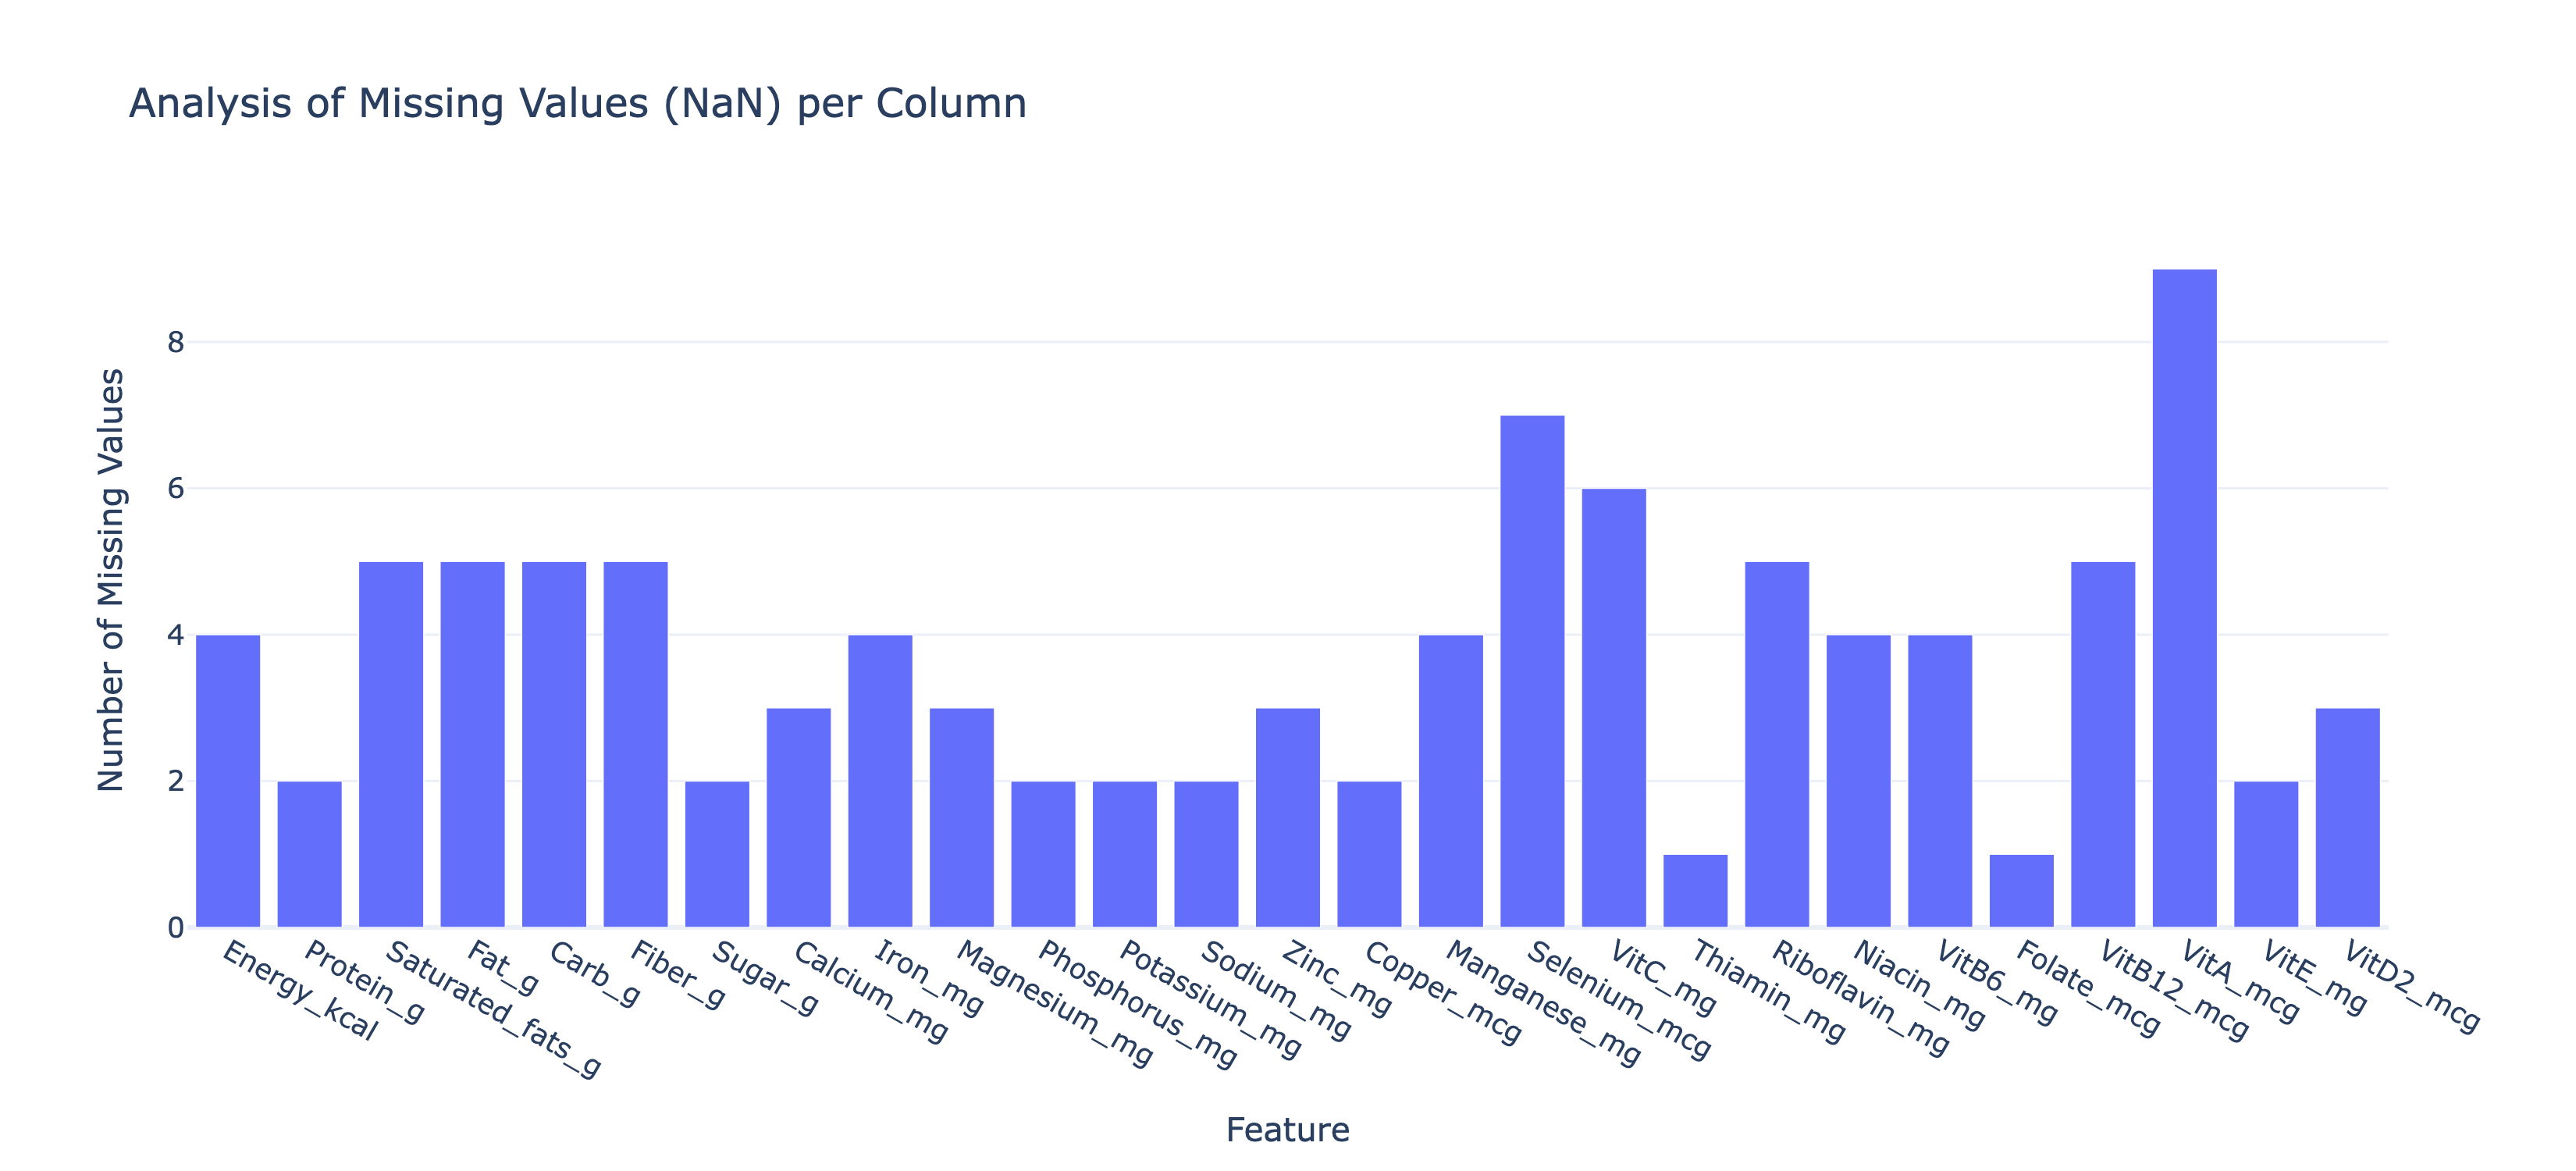
\includegraphics[width=\linewidth]{plots/nan_values.png}
    \caption{}
    \label{fig: missing_values}
\end{figure}

Následne sme roztriedili jedlá do kategórií podľa toho, aké slová obsahovali v atribúte \verb|Descrip|. Ich zastúpenie zobrazuje graf \ref{fig: category_hist}.

\begin{figure}[h!]
    \centering
    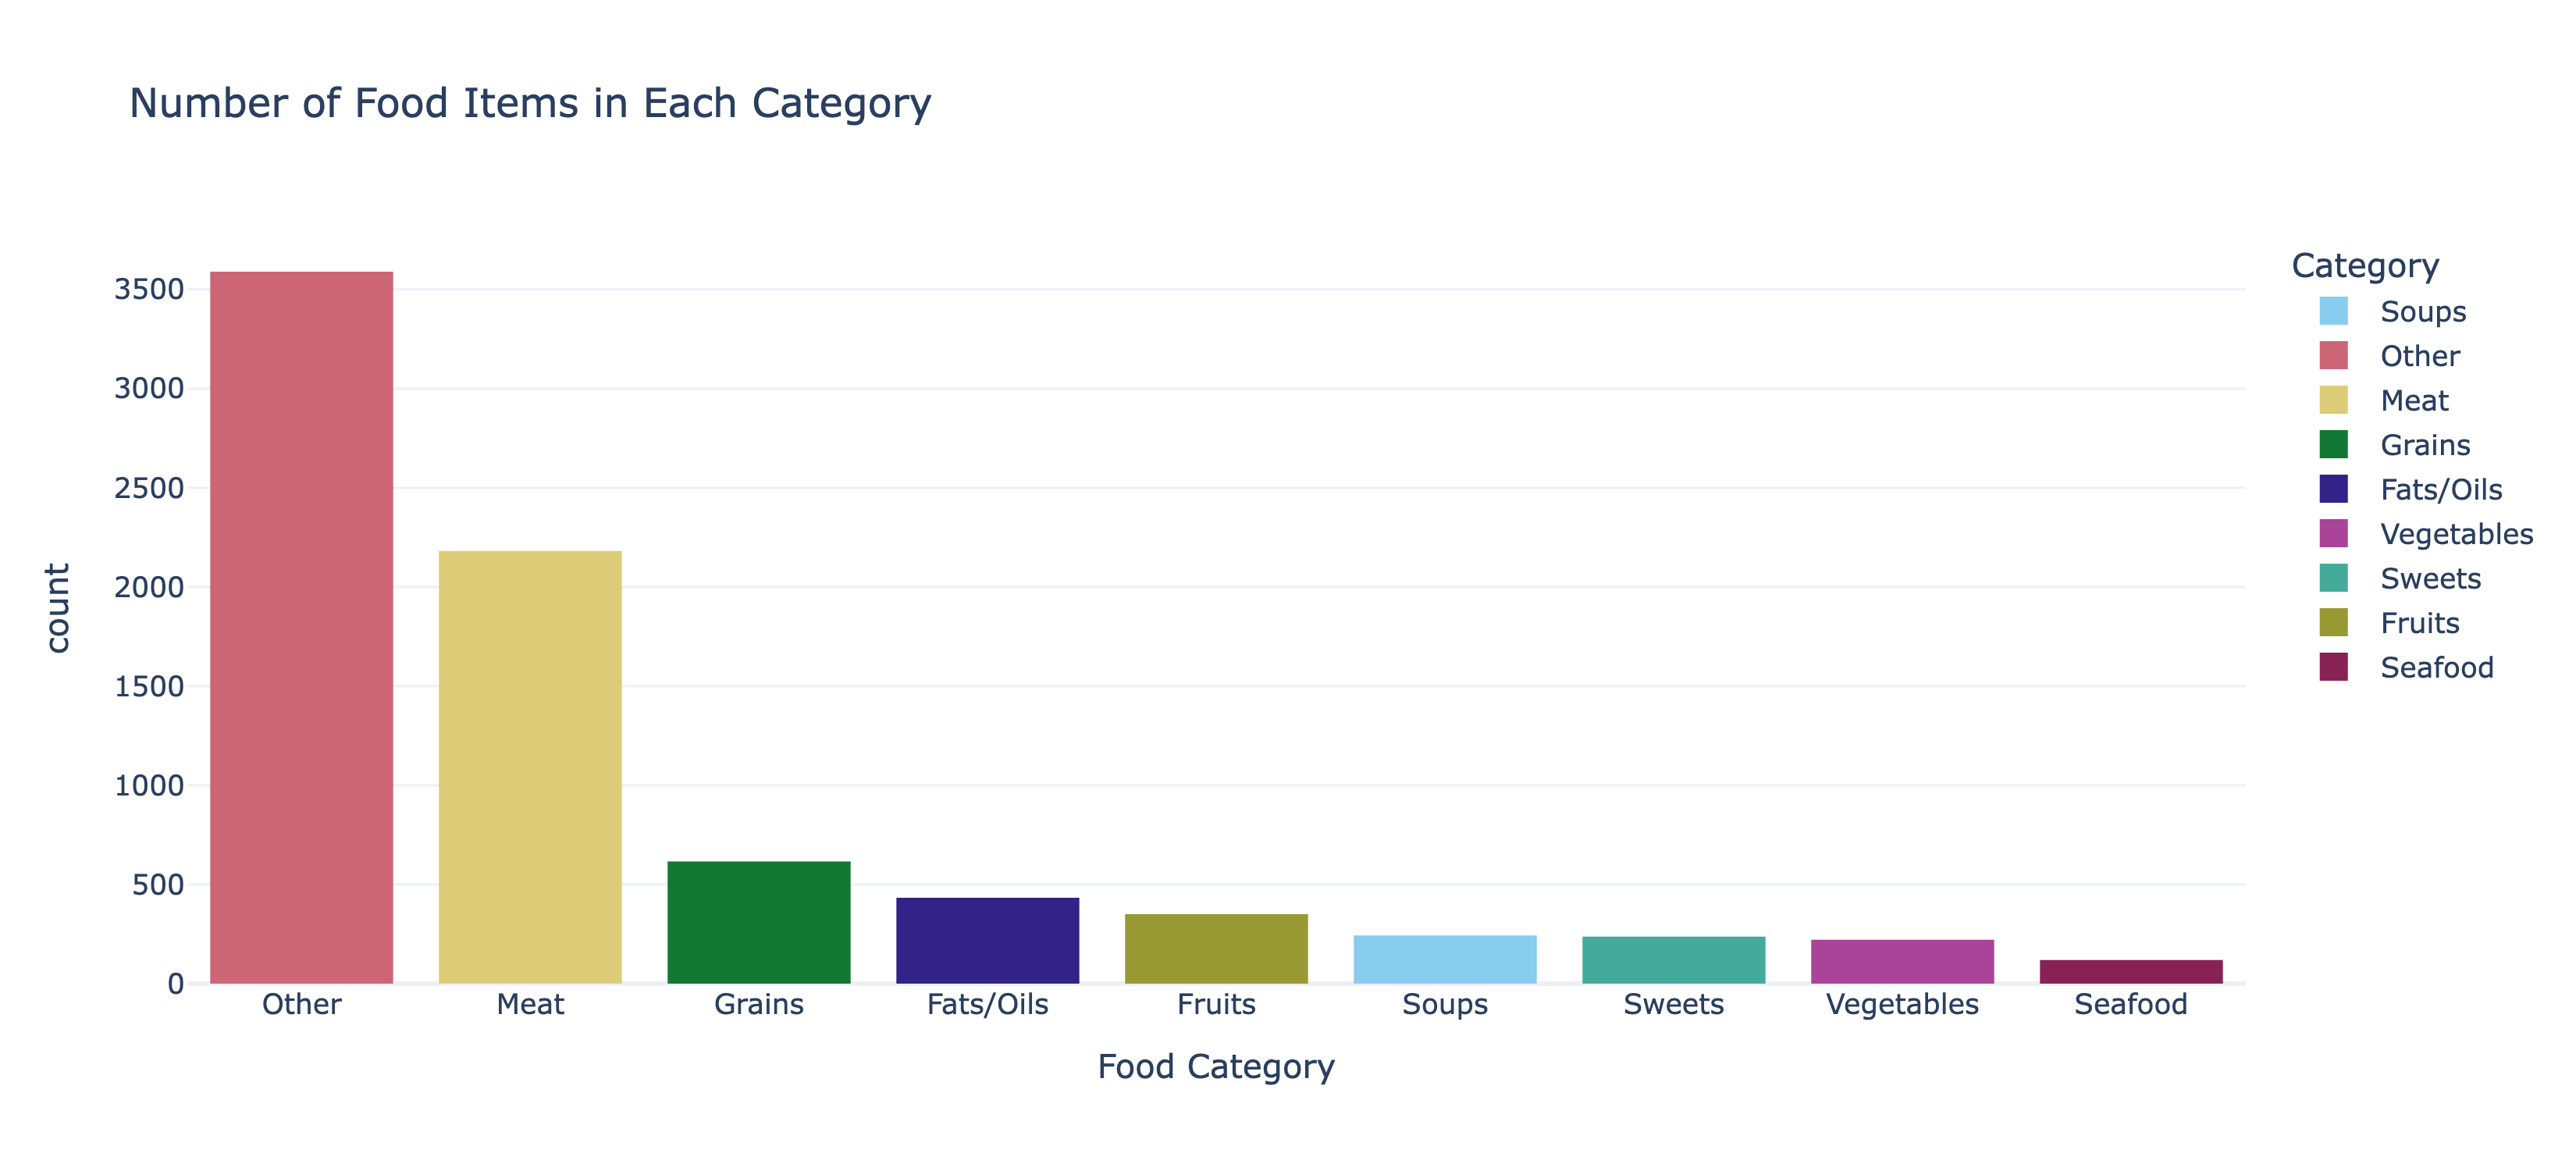
\includegraphics[width=\linewidth]{plots/category_hist.png} 
    \caption{}
    \label{fig: category_hist}
\end{figure}
\end{document}


